% !TEX root = ../main.tex
\vspace{-2mm}
\section{Inverse-distilled Diffusion Language Models}
\vspace{-2mm}
\label{sec:idlm}
  In this section, we present our core methodology for distilling a broad class of Diffusion Language Models into a few-step generator. Firstly, we provide the theoretical foundations supporting the extension of the Inverse Distillation framework to the discrete domain (\wasyparagraph\ref{sec:theoretical extension idlm}). We then address the practical challenges arising from the non-smooth nature of discrete spaces (\wasyparagraph\ref{sec:practical extension of idlm}). Lastly, we outline key implementation details (\wasyparagraph\ref{sec:technical aspects}).
  % However, a key challenge lies in the fact that existing training losses across prior models are formulated using different objective forms and parameterizations. 
  % To enable a unified application of Inverse Distillation, we first establish a general functional formulation of training objectives in \wasyparagraph~\ref{sec:unversal loss} and relate it to previous work. 
  % Building upon this foundation, 
  % We introduce our Inverse Distillation method in (\wasyparagraph\ref{sec:extension idlm}), followed by a discussion of practical implementation details in (\wasyparagraph\ref{sec:practical aspects}). 

\vspace{-1mm}
\subsection{Theoretical extension of Inverse Distillation}
\vspace{-1mm}
\label{sec:theoretical extension idlm}
  % All considered frameworks of discrete diffusion models (SEDD, MDLM, DUO) train either denoiser $\widehat{x}_0(x_t, t)$ or score function $\widehat{s}(x_t, t)$ using according loss function for it.
  % The methods SEDD~\eqref{eq:sedd loss}, MDLM~\eqref{eq:mdlm loss}, and Duo~\eqref{eq:duo loss} propose training a model parameterized either as a denoising function $\widehat{x}_0(x_t, t)$ or as a score function $\widehat{s}(x_t, t)$. To present the distillation framework in a unified manner, we introduce the notation $\widehat{f}(x_t, t)$ to represent a generic parameterized function, which may correspond to either $\widehat{s}$ or $\widehat{x}_0$.
  % and call it \textbf{teacher model}.
  % following standard notation of diffusion distillation papers. 
  % In the same way we denote $\LC_{\text{teach.}}$ as functional using to train these models, i.e. either $\LC_{\text{SEDD}}, \LC_{\text{MDLM}}, \LC_{\text{Duo}}$. Thus, diffusion language models consider problem:

\ecoparagraph{Unified notations.}
  SEDD~\eqref{eq:sedd loss}, MDLM~\eqref{eq:mdlm loss}, and Duo~\eqref{eq:duo loss} introduce different training objectives $\{\LC_{\text{SEDD}}, \LC_{\text{MDLM}}, \LC_{\text{Duo}}\}$ 
  and model parameterizations $\{\widehat{s}(x_t,t), \widehat{x}_0(x_t,t)\}$.
  To describe the distillation framework in a unified fashion, we use $\LC \in \{\LC_{\text{SEDD}}, \LC_{\text{MDLM}}, \LC_{\text{Duo}}\}$ to denote the diffusion training objective and introduce $\widehat{f}(x_t,t) \in \{\widehat{s}(x_t,t), \widehat{x}_0(x_t,t)\}$ as a parameterized function encompassing the relevant model parameterizations. Following the standard notation commonly adopted in diffusion distillation literature, we define the \textbf{teacher} model as:
  \begin{equation}
    f^* = \arg\min\nolimits_{\widehat{f}} \EE_{p^*(x_0)} \left[\LC(\widehat{f}, x_0)\right] \nonumber.
  \end{equation}
  % To model a complex data distribution $p^*(x_0)$, one typically trains a teacher model $f^* = \arg\min_{\widehat{f}} \LC_{\text{teach.}}(\widehat{f}, p^*)$  using objective for teacher training~\eqref{eq:forward optimization problem}, and then generates samples via a multi-step sampling procedure~\eqref{eq:backward diffusion}. 
% \vspace{-0.2mm}
\ecoparagraph{Inverse distillation for DLMs.}
  To address the issue of slow inference, we extend the Inverse Distillation framework, originally developed for continuous diffusion models, to the domain of Diffusion Language Models.
  % To do so, we need: 
  % \begin{itemize}
  %   \item (a) propose a new distillation objective for discrete diffusion models \eqref{eq:inverse discrete diffusion distillation}.
  %   \item (b) prove that the minimization of this objective leads to a model that correctly models data distribution (Theorem~\ref{thm:unique solution}).
  %   \item (c) propose a practical procedure to optimize this new objective (\wasyparagraph~\ref{sec:practical aspects}).
  % \end{itemize}
  % In this section, we cover theoretical aspects, i.e., points (a) and (b), while practical aspects are covered in \wasyparagraph~\ref{sec:practical aspects}. 
  Specifically, we consider a \textbf{student} model defined by a generator ${G_{\theta}\colon \ZC \to \VC}$, parameterized by parameters $\theta$, which transforms latent variables from a latent space $\ZC$ to a discrete output space $\VC$. The latent space $\ZC$ is equipped with a tractable prior distribution $p_{\ZC}$, inducing a distribution $p_{\theta}$ over $\VC$ via the mapping $G_{\theta}$. Then, following the logic of the continuous case, we propose to consider the following objective for the discrete diffusion:
  % We start by considering the following objective, similar to the continuous case:
  
  % To avoid the time-consuming sampling, we propose to train a student generator  $G_{\theta}\colon \ZC \to \VC$, parameterized by $\theta$, to approximate $p^*(x_0)$ directly. The generator defines a distribution $p^\theta$ by pushing forward a tractable reference distribution $p^{\ZC}$ over the latent space $\ZC$, \rewriteit{i.e., $p^\theta = G_\theta \# p^{\ZC}$}. Our key idea is to frame the training of the student generator as an instance of inverse distillation, where the parameters are represented as distributions $p^\theta$, and the goal is to find a distribution $p^{\theta^*}$ for which the solution to the forward optimization problem coincides with the teacher model, i.e., $f^* = \arg\min_{\widehat{f}} \LC_{\text{FOP}}(\widehat{f}, p^{\theta^*})$. Applying the inverse optimization objective in equation~\eqref{eq:inverse optimization problem} yields the following \textit{Inverse distilled Diffusion Language Models} (IDLM) loss:
  \begin{Box1}{IDLM loss, $\LC_{\text{IDLM}}(\theta) \vcentcolon=$}
    \vspace{-2pt}
    \begin{equation}
      \label{eq:inverse discrete diffusion distillation}
      \!\!\!\! \mathop{\EE}_{p_{\theta}(x_0)} \! \Big[\LC(f^*, x_0)\Big]
      - \min_{\widehat{f}}\! \mathop{\EE}_{p_{\theta}(x_0)}\! \Big[\LC(\widehat{f}, x_0)\Big],\!
    \end{equation}
  \end{Box1}
  where the second term includes training of \textbf{fake} model using the same loss as the teacher model, but with data $p_{\theta}(x_0)$ produced by the generator $G_{\theta}$.

\ecoparagraph{Theoretical validity of the training objective.}
  However, simply formulating this objective in a manner analogous to the distillation loss used in continuous diffusion models does not guarantee the validity of its solutions. While the loss function admits a trivial minimizer $\theta^*$ satisfying $p_{\theta^*} = p^*$, the absence of a uniqueness guarantee implies that the optimization procedure may converge to suboptimal solutions. Consequently, it is essential to establish that the \underline{minimizer recovers the true data distribution, i.e., ${p_{\theta^*} = p^*}$}. To address this, we present the following theorem. 

  % However, . While the loss function admits a trivial minimizer $\theta^*$ satisfying $p^{\theta^*} = p^*$, the absence of a uniqueness guarantee implies that the optimization procedure may converge to suboptimal solutions. Consequently, it is essential to establish that the \underline{minimizer recovers the true data distribution, i.e., ${p_{\theta}^* = p^*}$}. This condition constitutes a key theoretical requirement for validating the soundness of the proposed objective. To address this, we present the following theorem.
  
  % While this loss admits a trivial solution at $\theta^*$ such that $p^{\theta^*} = p^*$, the uniqueness of this solution is not guaranteed. As a result, optimization may converge to suboptimal solutions. To address this, the following theorem establishes a connection between $\LC_{\text{IDLM}}$ and the KL divergence $\DC_{\text{KL}}$.
  \begin{theorem}[Unique solution]
  \vspace{-1mm}
  \label{thm:unique solution} 
    For the SEDD~\eqref{eq:sedd loss}, MDLM~\eqref{eq:mdlm loss}, and Duo~\eqref{eq:duo loss} (in the limit as $\tau \to 0^{+}$) objectives the IDLM loss defined in equation~\eqref{eq:inverse discrete diffusion distillation} satisfies
    \begin{equation}
      \LC_{\text{IDLM}}(\theta) \geq \mathcal{D}_{\text{KL}}(p_{\theta} \parallel p^*)\geq 0 \nonumber
    \end{equation}
    and achieves its minimum (zero) if and only if the model distribution matches the target distribution
    \vspace{-2mm}
    \begin{equation}
      \LC_{\text{IDLM}}(\theta) = 0 \iff p_{\theta} = p^*. \nonumber
    \end{equation}
    \vspace{-2mm}
  \end{theorem}
  \vspace{-5mm}
  
  %
  We give the proof in Appendix~\ref{app: proof of the theorem}.

% \subsubsection{Student Generator $G_\theta$ Parameterization}


% We define the generator $G_\theta: \mathcal{Z} \to \Delta$ as a deterministic map designed to transport a tractable
% reference measure onto the geometry of the probability simplex. Here, $\mathcal{Z}$ represents the continuous latent space—typically $\mathbb{R}^d$ equipped with a standard Gaussian measure $p^\mathcal{Z}$—and $\Delta$ denotes the probability simplex in $\mathbb{R}^N$, representing the set of valid probability vectors over $N$ tokens.

% This mapping induces a model distribution $p^\theta$ on the simplex, characterized as the pushforward of the latent prior. Mathematically, this is expressed as:
% $$
% p^\theta \vcentcolon= (G_\theta)_\# p^\mathcal{Z}.
% $$
% Here, the notation $(G_\theta)_\#$ represents the pushforward of the measure $p^\mathcal{Z}$ by the measurable map $G_\theta$. This operator transports probability mass from the latent space to the output space, ensuring that for any measurable set $A \subseteq \Delta$, the induced probability is given by $p^\theta(A) \vcentcolon= p^\mathcal{Z}(G_\theta^{-1}(A))$.

% A critical aspect of this framework is the continuous relaxation of the discrete data structure. While the true data distribution $p^*$ is supported strictly on the vertices $\mathcal{V}$ (corresponding to discrete one-hot vectors), the generator $G_\theta$ maps latent points into the continuous *interior* of $\Delta$. This relaxation is essential, as it renders the mapping differentiable with respect to the parameters $\theta$. In the context of Inverse Distillation, $G_\theta$ parameterizes the student distribution; the training objective $\LC_{\text{IDLM}}(\theta)$ is consequently formulated to minimize the discrepancy between diffusion trajectories generated by this relaxed induced measure $p^\theta$ and those arising from the true data distribution $p^*$.



%   \begin{algorithm}[t]
%     \caption{Inverse distilled Diffusion Language Models (IDLM)}\label{alg:id3}
%     \SetKwInOut{Input}{Input}\SetKwInOut{Output}{Output}
%     \Input{Teacher network $f^{*}$; \\
%     Forward Optimization Loss $\LC_{\text{RFOP}}$; \\
%     Samples from target distribution $p^*(x_0)$; \\
%     Number of student iterations $K$;
%     }
%     \Output{Learned generator $G_{\theta}$}
    
%     \SetKwProg{samplelatent}{func}{}{}
%     \samplelatent{$\operatorname{MultiStepSampling}(p^*):$}{
%         $x_0 \sim p^*(x_0)$ \\
%         $t \sim \UC[0, T]$ \\
%         $x_{t} \sim p_{t \mid 0}(x_{t}\mid x_0)$ \tcp{Eq.~\eqref{eq:conditional_distribution}}
%         \KwRet $x_{t}, t$ 
%     }{}
%     \tcp{Initialize both generator and fake models from teacher model}
%     $G_\theta \gets \operatorname{CopyWeights}(f^*)$ \tcp*{Outputs to simplex $\Delta$}
%     $\widehat{f} \gets \operatorname{CopyWeights}(f^*)$
    
%     \For{$k = 1$ \KwTo $K$}{
%         \tcp{Update fake model}
%         $x_{t'}, t' \gets \operatorname{MultiStepSampling}(p^*)$ \\
%         $\LC_{\widehat{f}} \gets \LC_{\text{RFOP}}(\widehat{f}, G_{\theta}(x_{t'}, t'))$ \tcp{Eq.~\eqref{eq:relaxed forward optimization problem}} 
%         Update $\widehat{f}$ by using $\frac{\partial \LC_{\widehat{f}}}{\partial \widehat{f}}$
        
%         \tcp{Update student model}
%         $x_{\tilde{t}}, \tilde{t} \gets \operatorname{MultiStepSampling}(p^*)$ \\
%         $\LC_{\text{IDLM}}(\theta) \gets \Big[\LC_{\text{RFOP}}(f^*, G_{\theta}(x_{\tilde{t}}, \tilde{t})) - \LC_{\text{RFOP}}(\widehat{f}, G_{\theta}(x_{\tilde{t}}, \tilde{t}))\Big]$ \tcp{Eq.~\eqref{eq:inverse discrete diffusion distillation}} 
%         Update $G_{\theta}$ by using $\frac{\partial \LC_{\text{IDLM}}(\theta)}{\partial \theta}$
%     }
%   \end{algorithm}
  
  \begin{figure*}[ht!]
    \centering
    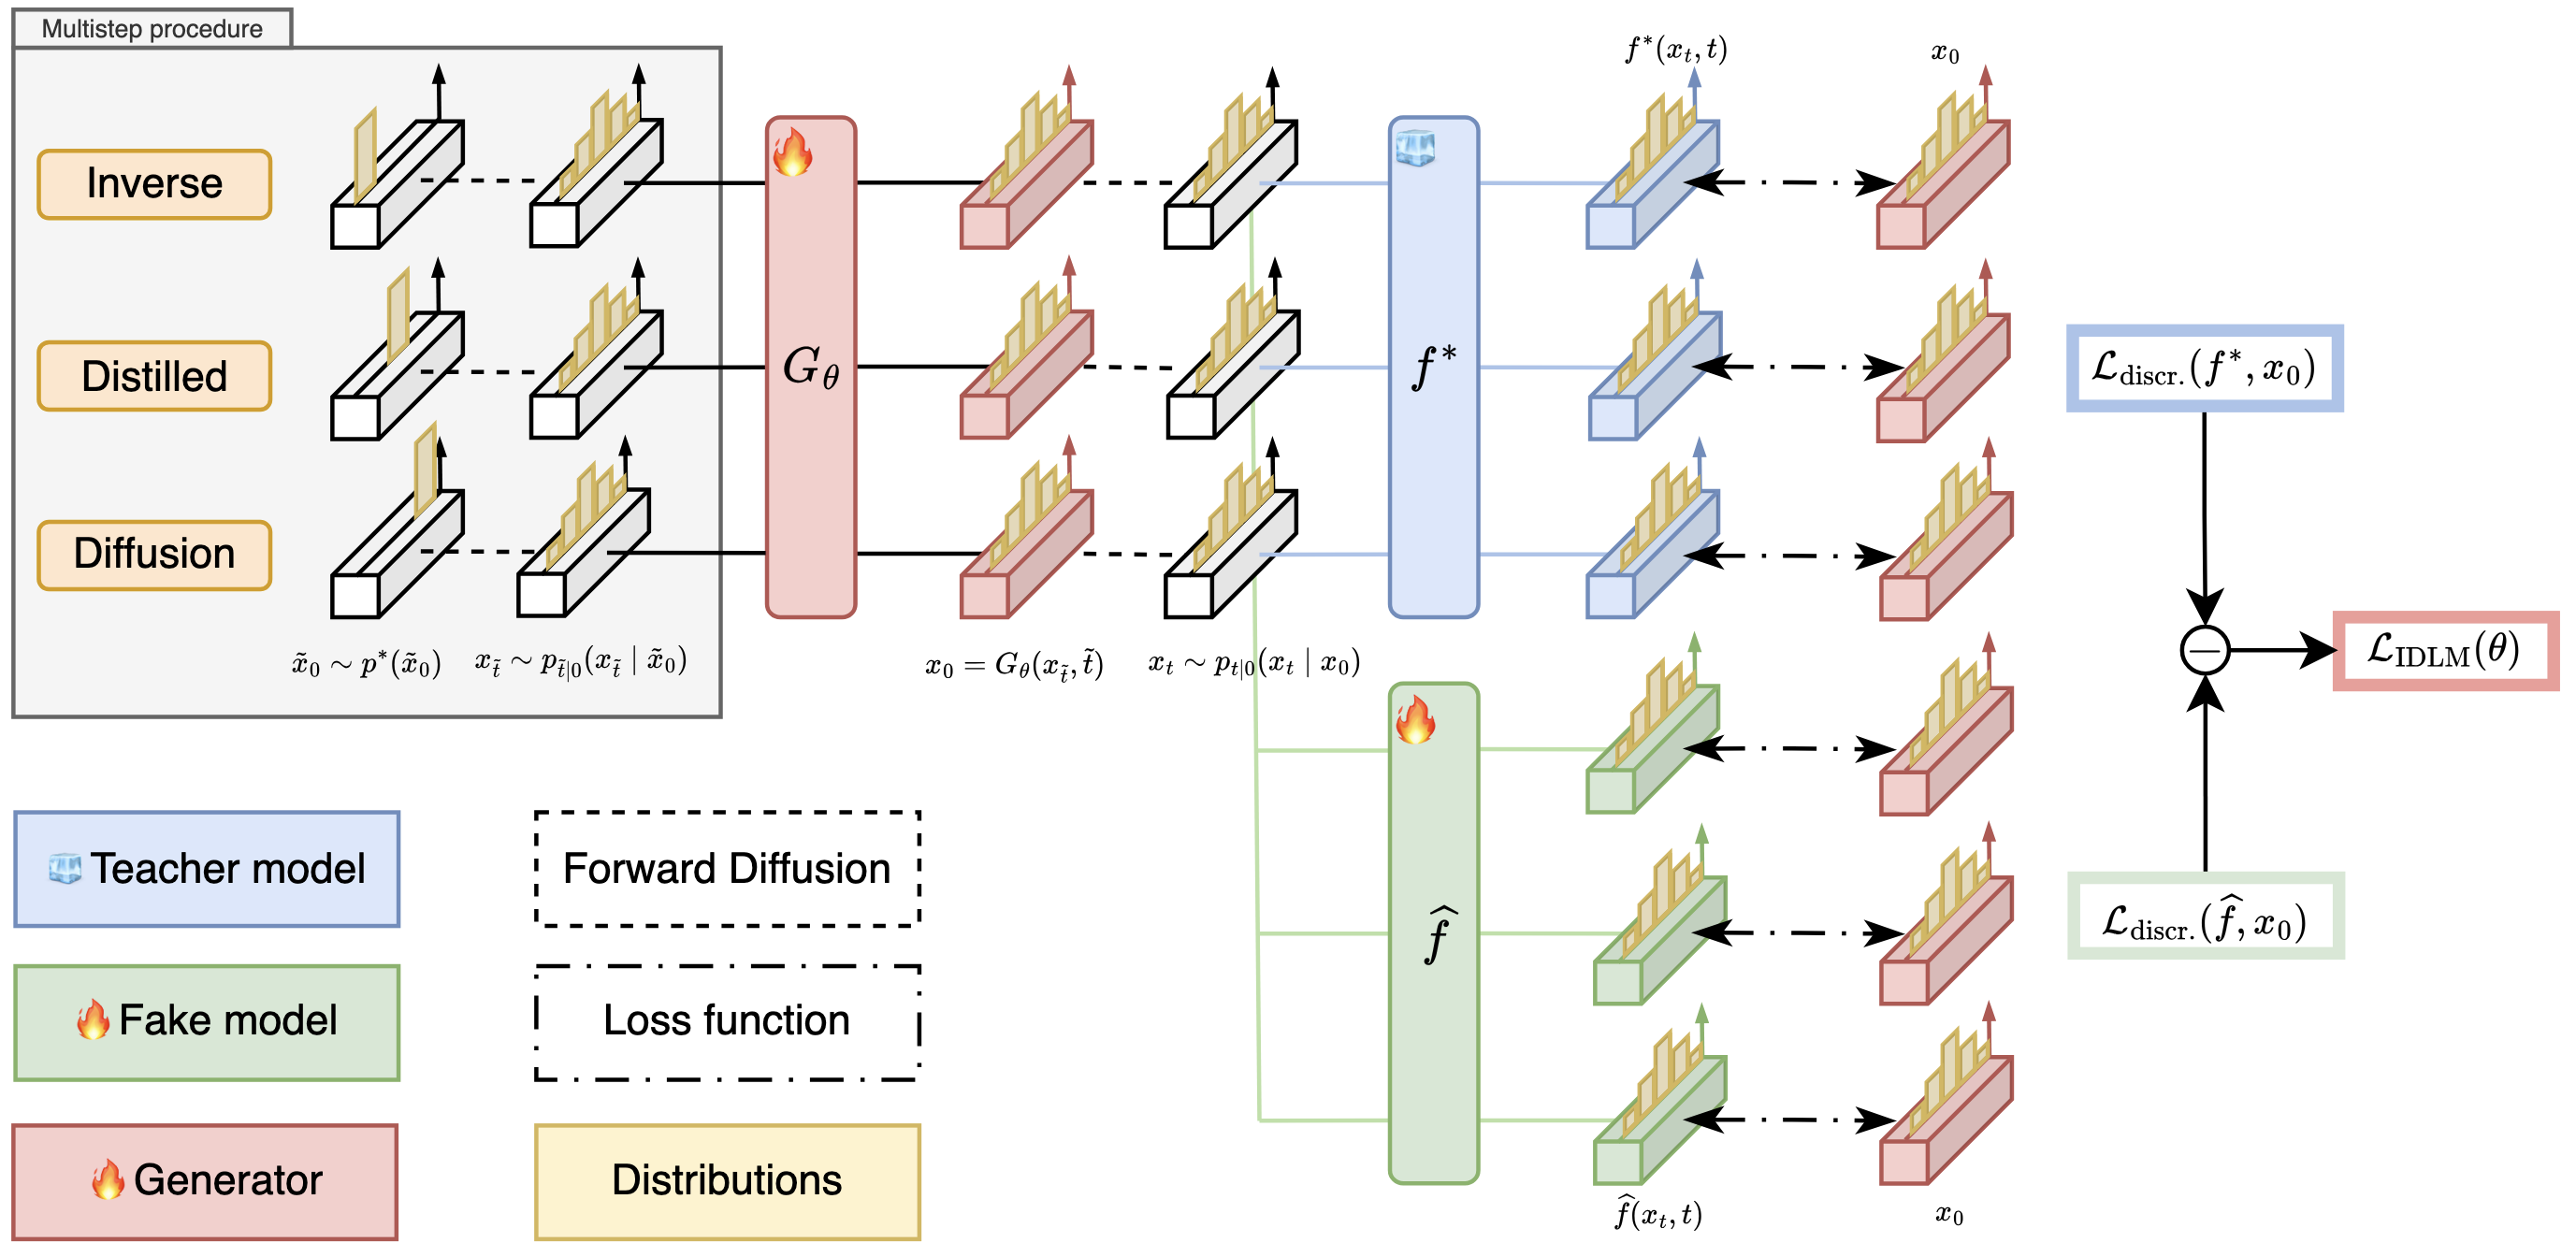
\includegraphics[width=0.82\linewidth]{images/method.png}
    % \caption{TODO: Overview of IDLM. We distill a pre-trained discrete diffusion teacher into a student generator. Crucially, to address the non-differentiability of discrete data, our student generator $G_\theta$ outputs a continuous probability vector on the simplex $\Delta$. This allows gradients to flow from the inverse distillation loss through the forward diffusion process back to the generator parameters $\theta$, enabling stable end-to-end training.}
    \caption{\textbf{Overview of our Inverse-Distilled Diffusion Language Model (IDLM) framework.} The objective is to distill a pretrained Diffusion Language Model $f^*$, referred to as the \textbf{teacher}, into a few-step generator $G_{\theta}$, referred to as the \textbf{student}. To this end, we extend the concept of \emph{Inverse Distillation}, originally developed for continuous diffusion models, to the discrete domain. The training procedure involves a nested optimization scheme: an auxiliary diffusion model $\widehat{f}$ (the \textbf{fake} model), is optimized using the same training loss as the teacher, but with data generated by the student $G_{\theta}$. Subsequently, the generator is updated using the IDLM objective introduced in (\wasyparagraph\ref{sec:theoretical extension idlm}).}
    \label{fig:method}
    \vspace{-5mm}
  \end{figure*}

% \label{sec:practical aspects}
%   While the theoretical foundations of the method have been established, a direct implementation of the IDLM loss for discrete diffusion models is not feasible in practice due to two primary challenges:
%   \begin{itemize}
%     \item The IDLM objective \eqref{eq:inverse discrete diffusion distillation} is not differentiable since it includes distribution $p_{\theta}$ parametrized by a discrete generator $G_{\theta}$. 
%     % gradients must pass through discrete sampling steps, $x_0 \sim p^{\theta}(x_0)$ and $x_t \sim p_{t \mid 0}(x_t \mid x_0)$.
%     \item Distilling teacher diffusion $f^*$ into a one-step generator $G_{\theta}$ for text generation, is practically challenging due to limited model capacity and the difficulty of learning a direct mapping from latent space to diverse, high-quality text.
%   \end{itemize}
%   %
%   To address these issues, we first propose a solution to the gradient estimation challenge in Section~\ref{sec:gradients}. Then, motivated by the second limitation, we extend the IDLM framework to support multi-step generation in Section~\ref{sec:multistep}. Finally, we summarize the method in Section~\ref{sec:algorithm}.

\vspace{-2mm}
\subsection{Practical extension of Inverse Distillation}
\label{sec:practical extension of idlm}
\vspace{-2mm}
Although we have theoretically established the validity of the proposed inverse distillation objective IDLM~\eqref{eq:inverse discrete diffusion distillation}, the discrete nature of the output space $\VC$ continues to pose significant practical challenges for the gradient-based optimization. 
In particular, the IDLM loss contains two primary bottlenecks. (i) First, the student generator ${G_{\theta} \colon \ZC \to \VC}$ produces outputs in the one-hot space $\VC$, which in practice necessitates the use of unstable techniques, such as the hard Gumbel-Softmax, thereby complicating gradient propagation. (ii) Second, samples $x_t \sim p_{t \mid 0}(x_t \mid x_0)$ depend on $x_0$, and thus implicitly on $\theta$. This introduces an additional challenge, as differentiating through the sampling operation $\sim$ is nontrivial in the discrete setting. Below we mitigate these challenges and develop a feasible training procedure.

\ecoparagraph{(i) Simplex relaxation.}
\label{sec:simplex relaxation}
To address the first challenge, we relax the output space of the student generator from the discrete set $\VC$ to the probability simplex $\Delta$, and accordingly redefine the generator as $G_{\theta}\colon \ZC \to \Delta$. This relaxation enables smooth gradient flow but introduces a nontrivial question regarding the computation of the training objective, since the generator outputs no longer lie in the original discrete space. Specifically, under this reparameterization, the IDLM objective becomes:
\begin{gather}
  \LC_{\text{IDLM}}(\theta)
  \!=\! \EE_{p_{\theta}(x_0)}\!\Bigl[\LC(f^*, x_0) - \min_{\widehat{f}}\LC(\widehat{f}, x_0)\Bigr]\!=
  \nonumber \\
  = \EE_{p_{\ZC}(z)}\!\Bigl[\LC(f^*, G_{\theta}(z)) - \min_{\widehat{f}}\LC(\widehat{f}, G_{\theta}(z))\Bigr],
  \nonumber
\end{gather}
where $z \sim p_{\ZC}(z)$ denotes a latent variable. Since $x_0$ appears only within the teacher loss $\LC$, we must ensure that this loss remains computable when substituting discrete samples $x_0 \in \VC$ with relaxed outputs $G_{\theta}(z) \in \Delta$. To this end, we note that all teacher losses under consideration $\LC \in \{\LC_{\text{SEDD}}, \LC_{\text{MDLM}}, \LC_{\text{Duo}}\}$ incorporate $x_0$ in one of two mathematically compatible forms: (i) through scalar products $\langle \cdot, x_0 \rangle$, or (ii) via the distribution $p_{t|0}(\cdot \mid x_0)$, which can be expressed as a matrix-vector product:
\begin{gather}
    p_{t \mid 0}(\cdot \mid x_0) = \exp\left(\bar{\sigma}_t Q\right)x_0.
    \nonumber
\end{gather}
%
Consequently, each of the considered teacher losses is mathematically well-defined not only for one-hot vectors from $\VC$ but also for any input from the probability simplex $\Delta$. This reparameterization enables end-to-end training of the generator using standard differentiable operations, such as the $\softmax$ function, thereby avoiding the need for unstable discrete relaxation methods like the hard Gumbel--Softmax.
% We address the first challenge by relaxing the output space of the student generator from the discrete set $\VC$ to the probability simplex $\Delta$, and accordingly redefining the generator as $G_{\theta} \colon \ZC \to \Delta$. However, this relaxation raises nontrivial validity concerns, as the resulting outputs no longer lie in the original discrete domain. In particular, under this reparameterization, the IDLM objective becomes
% \begin{gather}
%     \LC_{\text{IDLM}}(\theta)
%     = \EE_{p_{\theta}(x_0)}\!\left[\LC_{\text{teach.}}(f^*, x_0) - \min_{\widehat{f}}\LC_{\text{teach.}}(\widehat{f}, x_0)\right]
%     \nonumber \\
%     = \EE_{p_{\ZC}(z)}\!\left[\LC_{\text{teach.}}(f^*, G_{\theta}(z)) - \min_{\widehat{f}}\LC_{\text{teach.}}(\widehat{f}, G_{\theta}(z))\right],
%     \nonumber
% \end{gather}
% where $z \sim p_{\ZC}(z)$ denotes the latent variable. It is therefore necessary to ensure that replacing discrete samples $x_0 \in \VC$ with their relaxed counterparts $G_{\theta}(z) \in \Delta$ preserves the validity of the teacher loss $\LC_{\text{teach.}}$.
% $\LC_{\text{IDLM}}(\theta)$.
% While we theoretically established validity of novel extended inverse distillation objective \eqref{eq:inverse discrete diffusion distillation}, the practical question of using this objectives remains. Specifically, it is not clear how to efficiently use gradient-based optimization methods for objective which includes sampling from the discrete $p_{\theta}(x_0)$.
% We start from the differentiation of the $\LC_{\text{IDLM}}$. 
% % We remind, that:
% % $$
% %     x_0 = G_{\theta}(z), \quad z \sim p(z).
% % $$
% \begin{gather}
%     \nabla_{\theta} \LC_{\text{IDLM}}(\theta) = \nabla_{\theta} \EE_{x\sim p_{\theta}}\left[\LC_{\text{teach.}}(x, f^*) - \LC_{\text{teach}}(x, f_{\phi^*}) \right] = 
%     \nonumber
%     \\
%     \nabla_{\theta} \EE_{z \sim p(z)}\left[\LC_{\text{teach.}}(G_{\theta}(z), f^*) - \LC_{\text{teach}}(G_{\theta}(z), f_{\phi^*}) \right] = 
%     \nonumber
%     \\
%     \EE_{z\sim p(z)}\left[\nabla_{x_0}(\LC_{\text{teach.}}(x_0, f^*) - \LC_{\text{teach.}}(x_0, f_{\phi^*}))\frac{dG_{\theta}}{d\theta}\right ]_{x_0=G_{\theta}(z)}
%     \nonumber
% \end{gather}
% Since $G_\theta$ outputs discrete one-hot tokens, it is non-differentiable (or piece-wise constant), so the gradient $\frac{dG_{\theta}}{d\theta}$ vanishes / is undefined. 
% To overcome this problem we use a simplex relaxation ${x_0=G_\theta(z)\in\Delta}$, i.e. parametrize the generator $G_{\theta}$ to output samples on the simplex.
% Furthermore, 
% and extend $\LC_{\text{teach}}$ to the simplex, enabling standard backpropagation.
% The gradient $\nabla_\theta \LC_{\text{IDLM}}(\theta)$:
% involves differentiating through the expectation over $x_0 \sim p^\theta$ and $x_t \sim p_{t|0}(\cdot | x_0)$. In the IDLM loss~\eqref{eq:inverse discrete diffusion distillation}, two primary sources of gradient flow complexity arise from these sampling steps, both of which depend on the generator parameters $\theta$. Since gradients must propagate through both the distributions and their corresponding samples, this results in four critical gradient pathways:
% \vspace{-1em}
% \begin{equation}
%     \label{eq:gradient_decomposition}
%     \begin{split}
%     \nabla_\theta \LC_{\text{IDLM}} &= \underbrace{\frac{\partial \LC}{\partial p^\theta} \cdot \frac{\partial p^\theta}{\partial \theta}}_{\text{(I)}} + \underbrace{\frac{\partial \LC}{\partial x_0} \cdot \frac{\partial x_0}{\partial \theta}}_{\text{(II)}} \\
%     &\quad + \underbrace{\frac{\partial \LC}{\partial p_{t|0}} \cdot \frac{\partial p_{t|0}}{\partial \theta}}_{\text{(III)}} + \underbrace{\frac{\partial \LC}{\partial x_t} \cdot \frac{\partial x_t}{\partial \theta}}_{\text{(IV)}}.
%     \end{split}
% \end{equation}
% \vspace{-1em}
% \ecoparagraph{Term (I): Generator Reparameterization ($\boldsymbol{\frac{\partial p^{\theta}}{\partial \theta}}$).}
% We employ a reparameterization strategy by expressing \rewriteit{$p^{\theta} = G_{\theta} \# p^{\ZC}$}, where the generator $G_{\theta}\colon \ZC \to \VC$ maps latent variables to the discrete output space. Under this formulation, expectations with respect to $p^{\theta}$ can be rewritten as expectations over the latent distribution $p^{\ZC}$ by setting $x_0 = G_{\theta}(z) \in \VC$ for $z \sim p^{\ZC}(z)$. This reparameterization allows gradients to propagate through the deterministic mapping $G_{\theta}$ and eliminates the need to compute the gradient $\frac{\partial p^{\theta}}{\partial \theta}$ directly. Thus, Term (I) vanishes.
% ($\boldsymbol{\frac{\partial x_0}{\partial \theta}}$).}
% While the generator parameterization $G_{\theta}\colon \ZC \to \VC$ is theoretically well founded, the discreteness of the output space $\VC$ poses challenges for gradient-based optimization. In particular, propagating gradients through discrete outputs requires approximation techniques such as the Gumbel--Softmax relaxation, which are often unstable and lead to high-variance gradient estimates.
% \subsubsection{Simplex Relaxation}
% \label{sec:simplex relaxation}
% To address this issue, 
% \begin{proposition}[Natural extention of ]
%   \label{thm:unique solution} 
%     Let $\PP$ denote the probability measure over trajectories of the diffusion process. We further denote by $\PP^{\theta}$ the trajectory distribution corresponding to the generator induced distribution $p^{\theta}$, and by $\PP^{*}$ the trajectory distribution corresponding to the target distribution $p^*$. Under this notation, for a broad class of Discrete Diffusion Models, the IDLM loss in equation~\eqref{eq:inverse discrete diffusion distillation} is equivalent to the following KL divergence objective:
%     \begin{equation*}
%       \LC_{\text{IDLM}}(\theta) = \DC_{\text{KL}} (\PP^{\theta} \parallel \PP^*).
%       \nonumber
%     \end{equation*}
%     Since the KL divergence admits a unique minimizer, this ensures the uniqueness of the solution and provides guarantees for recovering a valid result.
% \end{proposition}
% In order to resolve this concern, we note that all considered DLMs objectives $\LC_{\text{teach.}} \in \{\LC_{\text{SEDD}}, \LC_{\text{MDLM}}, \LC_{\text{Duo}}\}$, includes $x_0$ either in the form of scalar products $\langle \cdot, x_0 \rangle$ or in the form of a conditional forward distribution $p_{t|0}(\cdot|x_0)$, which in turn represented as matrx-vector product:
% \begin{gather}
%     p_{t \mid 0}(\cdot \mid x_0) = \exp\left(\bar{\sigma}_t Q\right)x_0 
%     \nonumber
% \end{gather}
% Thus, all considered $\LC_{\text{teach.}}$ are mathematically correctly defined not only for one-hot vector products from $\VC$, but also for any vector on a probability simplex ${\Delta.}$ 
% We use this observation and relax the output space of the generator from the discrete set $\VC$ to the probability simplex $\Delta$, redefining the generator as $G_{\theta}\colon \ZC \to \Delta$, i.e. $x_0 = G_{\theta}(z) \in \Delta$. The inverse loss $\LC_{\text{IDLM}}$ is given by:
% \begin{gather}
%     \LC_{\text{IDLM}}(\theta) = \EE_{p_{\theta}(x_0)}\left[\LC_{\text{teach.}}(f^*, x_0) - \LC_{\text{teach}}(f_{\phi^*}, x_0) \right] = 
%     \nonumber
%     \\
%     \EE_{p(z)}\left[\LC_{\text{teach.}}(f^*, G_{\theta}(z)) - \LC_{\text{teach}}(f_{\phi^*}, G_{\theta}(z)) \right] 
%     \nonumber
%     % \\
%     % \EE_{p(z)}\left[\nabla_{x_0}(\LC_{\text{teach.}}(x_0, f^*) - \LC_{\text{teach.}}(x_0, f_{\phi^*}))\frac{dG_{\theta}}{d\theta}\right ]_{x_0=G_{\theta}(z)},
%     % \nonumber
% \end{gather}
% This reparametrized form allows to backpropagate through relaxed generator $G_{\theta}$ without using unstable hard Gumbel-Softmax techniques and just leverage stable $\softmax$ function.
% \begin{gather}
%     \nabla_{\theta} \LC_{\text{IDLM}}(\theta) = \nabla_{\theta} \EE_{p_{\theta}(x_0)}\left[\LC_{\text{teach.}}(x, f^*) - \LC_{\text{teach}}(x, f_{\phi^*}) \right] = 
%     \nonumber
%     \\
%     \nabla_{\theta} \EE_{p(z)}\left[\LC_{\text{teach.}}(G_{\theta}(z), f^*) - \LC_{\text{teach}}(G_{\theta}(z), f_{\phi^*}) \right] = 
%     \nonumber
%     \\
%     \EE_{p(z)}\left[\nabla_{x_0}(\LC_{\text{teach.}}(x_0, f^*) - \LC_{\text{teach.}}(x_0, f_{\phi^*}))\frac{dG_{\theta}}{d\theta}\right ]_{x_0=G_{\theta}(z)},
%     \nonumber
% \end{gather}
% where $\nabla_{x_0}\LC_{\text{teach.}}$ is the gradient of the loss used for the teacher model over $x_0$. 

\ecoparagraph{(ii) Backpropagation through the sampling procedure.}
Since the second problem depends on the specific form of conditional distribution $p_{t \mid 0}(x_t \mid x_0)$, we analyze the relevant cases separately, focusing on the Duo and MDLM (SEDD with absorbing process) formulations.

% \textbf{Case of Duo}. The objective in Duo is given in equation~\eqref{eq:duo loss} as:
% Forward process sampling is performed in the following reparametrized form:
% \begin{gather}
%     x_t = \softmax\!\left(\frac{\tilde{\alpha}_t x_0 + (1 - \tilde{\alpha}_t^2)\epsilon}{\tau}\right).
% \end{gather}
% for some small $\tau$ which is gradually decreased to zero and schedule parameters $\widetilde{\alpha}$. Thus, for small $\tau$ backpropagation through the $\LC_{\text{Duo}}$ is also performed using reparametrization trick:
% \begin{gather}
%     \int_0^1 \EE_{\tilde{p}_{t\mid 0}(w_t\mid x_0)} g_{\text{Duo}}(h^{\text{hard}}_{w_t},x_0, \widehat{x}_0(h^{\text{soft}}_{w_t}, t))dt, \nonumber
% \end{gather}
% in this case we can use the standard reparametrization trick for gaussian distribution defining by
% $$
%     w_t(x_0, \epsilon) = \tilde{\alpha}_t x_0 + \sqrt{(1-\tilde{\alpha}_t^2)}\epsilon,
% $$ 
% where $\epsilon \sim \NC(\epsilon\mid 0, I)$ and we obtain:
% \begin{gather}
%     \int_0^1 \EE_{\NC(\epsilon|0, I)} g_{\text{Duo}}(h^{\text{hard}}_{w_t(x_0, \epsilon)},x_0, \widehat{x}_0(h^{\text{soft}}_{w_t(x_0, \epsilon)}, t))dt,
% \end{gather}
% thus eliminating the necessity of backpropagation through the sampling process of distribution in expectation, because $\epsilon\sim \NC(\epsilon\mid 0, I)$ does not depend on $x_0$.

\textbf{Case of Duo.} The training objective in the Duo setting is given in equation~\eqref{eq:duo loss} as $\LC_{\text{Duo}}(\widehat{x}_0, x_0)\vcentcolon=$
\begin{gather}
  \textstyle \int_0^1 \EE_{\tilde{p}_{t\mid 0}(w_t\mid x_0)} \left[g(x_t(w_t),x_0, \widehat{x}_0(x_t^{\tau}(w_t), t))\right]dt. \nonumber
\end{gather}
Here we can apply the standard reparameterization trick for Gaussians by expressing the latent variable $w_t$ as:
\begin{gather}
  \textstyle w_t(x_0, \epsilon) = \tilde{\alpha}_t x_0 + \sqrt{1 - \tilde{\alpha}_t^2} \, \epsilon,
\end{gather}
where $\epsilon \sim \NC(0, I)$ is sampled independently of $x_0$. Substituting this into the objective yields $\LC_{\text{Duo}}(\widehat{x}_0, x_0)\vcentcolon=$
\begin{gather}
  \textstyle \int_0^1 \EE_{\epsilon \sim \NC(0, I)} \, \left[g(x_t(w_t),x_0, \widehat{x}_0(x_t^{\tau}(w_t), t))\right] \, dt,
\end{gather}
which eliminates the need to differentiate through the sampling operation itself, as the randomness is now isolated in $\epsilon$, which is independent of $x_0$. This reparameterization thus enables gradient-based optimization of the Duo objective.

% \textbf{Case of MDLM}. In this case there is no reparametrization for $p(x_t|x_0)$.  However, we can leverage here the SUBS parameterization of MDLM model introduced in ~\citep[See Sction 3.2.3]{sahoo2024simple}. Specifically, for unmasked $x_t \neq m$, it is known that: (a) the optimal denoiser is $\widehat{x}_0(x_t, t) = x_t$, (b) that $x_t = x_0$ since the forward process can only transform $x$ to mask vector $m$. Hence $\widehat{x}_0(x_t, t) = x_t = x_0$ and:
% \begin{gather}
%     \LC_{\text{MDLM}}(x_0, x_0) = 0.
%     \nonumber
% \end{gather} 
% All nonzero contributions to the loss occur when $x_t = m$, but in this case $x_t$ does not depend on $x_0$
% for which conditional distribution $p_{t \mid 0}(x_t \mid x_0)$ reduces to a constant~\citep{sahoo2024simple}. 
% As a result, neither $p_{t \mid 0}(x_t \mid x_0)$ nor the sampled $x_t$ depends on $x_0$. 
% and there is no need to backpropagate through sampling of $p_{t|0}(x_t|x_0)$. Thus, one can write the objective $\LC_{\text{MDLM}}(\widehat{x}_0, G_{\theta}(z))$ as:
% \begin{gather}
%   \int_0^1 \, \EE_{p_{t|0}(x_t|\text{sg}(G_{\theta}(z)))} \left[
%       \lambda_t \langle \log\widehat{x}_0(x_t, t), G_{\theta}(z) \rangle
%   \right]dt.
%   \nonumber
% \end{gather}
% \begin{gather}
%      \int_0^1 \, \EE_{p_{t|0}(x_t|x_0)} \left[
%           \frac{\alpha_t'}{1 - \alpha_t} \nabla_{x_0}\langle \log\widehat{x}_0(x_t, t), x_0 \rangle
%       \right]dt
%     \nonumber
% \end{gather}
% Same is true for $\LC_{\text{SEDD}}$ with absorbing process, since for absorbing process $\LC_\text{SEDD}$ is equivalent to $\LC_{\text{MDLM}}$.

\textbf{Case of MDLM (SEDD absorbing).} In the case of MDLM, the forward transition distribution $p(x_t \mid x_0)$ does not admit a standard reparameterization. However, we can leverage the \textsc{subs} parameterization of the MDLM model introduced in~\citep[see Section 3.2.3]{sahoo2024simple}. Specifically, for unmasked tokens (i.e., $x_t \neq m$), the following properties hold: (a) the optimal denoiser satisfies $\widehat{x}_0(x_t, t) = x_t$, and (b) $x_t = x_0$, since the forward process either preserves the token or replaces it with a fixed mask token $m$. As a result, in this case, $\widehat{x}_0(x_t, t) = x_t = x_0$, and the loss becomes $\LC_{\text{MDLM}}(x_0, x_0) = 0.$
Thus, all nonzero contributions to the loss arise from instances where $x_t = m$. In this case, $x_t$ is independent of $x_0$, as the mask token is fixed and does not result from a stochastic transformation conditioned on $x_0$. Consequently, there is no need to backpropagate through the sampling of $p_{t \mid 0}(x_t \mid x_0)$. This allows us to rewrite the loss as:
\begin{gather}
  \textstyle \int_0^1 \, \EE_{p_{t \mid 0}(x_t \mid \text{sg}(G_{\theta}(z)))} \left[
  \lambda_t \, \langle \log \widehat{x}_0(x_t, t), G_{\theta}(z) \rangle
  \right] dt,
  \nonumber
\end{gather}
where $\text{sg}(\cdot)$ denotes the stop-gradient operator. This formulation enables efficient training without requiring differentiable sampling from the discrete forward process.


% Thus, the original gradient of $\LC_{\text{IDLM}}$ can be computed using automatic differentiation techniques.

% To conclude the derivation of the gradient, we consider $\nabla_{x_0}\LC_{\text{teach.}}$ case by case:
% This relaxation enables stable gradient-based optimization using the differentiable $\softmax$ function. 
% Unlike stochastic relaxations that introduce variance, this analytical extension provides a deterministic path for gradients. 

% \textbf{Teacher loss extentsion (simplex-valued $x_0$).} Teacher loss $\LC_{\text{teach.}}(x_0, f)$ given by \eqref{eq:forward optimization problem} under this relaxation naturally extends without any changes. Note, that all variants of teacher loss includes $x_0$ in one of three ways: through ${p_{t \mid 0}(x_t \mid x_0)}$, through matrxi-vector products (e.g. 

% Specifically, the conditional distribution ${p_{t \mid 0}(x_t \mid x_0)}$ in equation~\eqref{eq:conditional_distribution} remains well defined, as it corresponds to a matrix-weighted inner product with $x_0 \in \Delta.$ 

% \textbf{Teacher loss extentsion (simplex-valued $x_0$).} Teacher loss $\LC_{\text{teach.}}(x_0, f)$ given by \eqref{eq:forward optimization problem} under this relaxation naturally extends without any changes. Specifically, the conditional distribution ${p_{t \mid 0}(x_t \mid x_0)}$ in equation~\eqref{eq:conditional_distribution} remains well defined, as it corresponds to a matrix-weighted inner product with $x_0 \in \Delta.$ Similarly, the conditional function $f(x_t, t \mid x_0)$ remains well defined, as it either involves ratios of conditional distributions (in the SEDD case) or depends explicitly on $x_0$ (in the MDLM and UDLM settings).
% Crucially, under this extension the teacher objective~\eqref{eq:teacher_model_training}
% remains well-defined \emph{without any modifications}, because it depends on $x_0$
% only through matrix-vector products with $\tilde x_0$.
% Indeed, $p_{t|0}(\cdot\mid \tilde x_0)$ is given by $K_t\tilde x_0$,
% and the corresponding conditional targets admit the same property:
% \begin{itemize}
% \item \textbf{SEDD:} the conditional score uses only ratios of entries of $K_t\tilde x_0$, e.g.
% \[
% \langle s(x_t,t\mid x_0),y\rangle
% =\frac{\langle y,K_t x_0\rangle}{\langle x_t,K_t\tilde x_0\rangle},
% \]
% so it depends on $\tilde x_0$ only via the vector $K_t\tilde x_0$;
% \item \textbf{MDLM/UDLM:} the target is $x_0$ itself, which extends linearly to $\tilde x_0\in\Delta$,
% turning the per-token loss into a cross-entropy,
% \[
% \ell(\tilde x_0,\widehat x_0(x_t,t))
% = -\sum_{v=1}^N (\tilde x_0)_v \log \widehat x_{0,v}(x_t,t)
% = -\tilde x_0^\top \log \widehat x_0(x_t,t).
% \]
% \end{itemize}

% Similarly, the conditional function $f(x_t, t \mid x_0)$ remains well defined, as it either involves ratios of conditional distributions (in the SEDD case) or depends explicitly on $x_0$ (in the MDLM and UDLM settings).
% For the loss function, we must verify that it extends to $\tilde{x}_0 \in \Delta^{V-1}$. For MDLM, the loss takes the form:
% \begin{equation}
%     \label{eq:relaxed_mdlm_loss}
%     -\sum_{v \in \VC} (\tilde{x}_0)_v \log \hat{f}(m, t)_v = -\tilde{x}_0^\top \log \hat{f}(m, t),
% \end{equation}
% which is differentiable in $\tilde{x}_0$. Similar extensions hold for SEDD and UDLM.

% \textbf{Gradient of teacher objective.} Apart of computing $\frac{dG_{\theta}}{d\theta}$ the gradient involves computation of $\nabla_{x_0}\LC_{\text{teach.}}(x_0, f)$:
% \begin{gather}
%     \nabla_{x_0} \int_0^1 \!\! \EE_{p_{t|0}(x_t|x_0)} \!\! \sum_{y \neq x_t}\!  w_t \DC_{F\circ\psi_t}\!\left(f(x_t, t \!\mid\! x_0), \widehat{f}(x_t, t)\right) \!dt
%     \nonumber
% \end{gather}
% The main obstacle of computing this gradient over $x_0$ is taking the gradient over expectation over $p_{t|0}(x_t|x_0)$. 

% \ecoparagraph{Terms (III) and (IV): Process-Specific Estimation ($\boldsymbol{\frac{\partial p_{t \mid 0}}{\partial \theta}}$ and $\boldsymbol{\frac{\partial x_t}{\partial \theta}}$).}
% The conditional distribution $p_{t \mid 0}$ depends on the diffusion matrix and, consequently, on the specific diffusion process. This structure can be exploited to handle both gradient terms effectively. 

% \textbf{Case 1: Absorbing Process (MDLM).}
% In the case of the \underline{absorbing process} for unmasked $x_t \neq m$, it is known that: (a) the optimal denoiser is $\widehat{x}_0(x_t, t) = x_t$, (b) that $x_0 = x_t$ since the forward process can only transform $x$ to mask vector $m$. In this case:
% \begin{gather}
%     \langle\log\widehat{x}_0(x_t, t), x_0 \rangle = 0, \quad \text{and}\quad \LC_{\text{MDLM}}(\widehat{x}_0, x_0) = 0.
%     \nonumber
% \end{gather} 
% All nonzero contributions to the loss occur when $x_t = m$, for which conditional distribution $p_{t \mid 0}(x_t \mid x_0)$ reduces to a constant~\citep{sahoo2024simple}. As a result, neither $p_{t \mid 0}(x_t \mid x_0)$ nor the sampled $x_t$ depends on $x_0$. And $\nabla_{x_0} \LC_{\text{MDLM}} =$
% \begin{equation}
%      \int_0^1 \, \EE_{p_{t|0}(x_t|x_0)} \left[
%           \frac{\alpha_t'}{1 - \alpha_t} \nabla_{x_0}\langle \log\widehat{x}_0(x_t, t), x_0 \rangle
%       \right]dt
%     \nonumber
% \end{equation}
% Same is true for $\LC_{\text{SEDD}}$ with absorbing process, since for absorbing process $\LC_\text{SEDD}$ is equivalent to $\LC_{\text{MDLM}}$. Thus, the original gradient of $\LC_{\text{IDLM}}$ can be computed using automatic differentiation techniques.

% \textbf{Case 2: Uniform Process (UDLM/Duo).}
% For the \underline{uniform process}, we adopt the Diffusion Duality (Duo) formulation~\citep{sahoo2025the}, which establishes a connection between Gaussian and uniform diffusion processes through a reparameterization of the diffusion schedule, denoted by $\tilde{\alpha}_t \vcentcolon= \atnew^{-1}(\alpha_t)$. Under this formulation, the expectation over $p_{t \mid 0}(x_t \mid x_0)$ appearing in the loss can be replaced as an expectation over $\epsilon \sim \NC(0, I)$ via the change of variables $x_t = \lim_{\tau \to 0^+}\softmax\!\left(\frac{\tilde{\alpha}_t x_0 + (1 - \tilde{\alpha}_t^2)\epsilon}{\tau}\right).$
% In practice, we fix $\tau$ to a sufficiently small value, which yields a numerically stable $\softmax$ transformation and ensures that $x_t \in \Delta$. The gradient $\nabla_{x_0}\LC_{\text{Duo}}$ =:
% \begin{gather}
%     \nabla_{x_0}
%     \nonumber
% \end{gather}
% Importantly, within the Duo framework, the teacher model is parameterized as $f\colon \Delta \times [0, T] \to \Delta$, and therefore naturally accepts inputs from the simplex, allowing gradients to propagate through $x_t$ in a stable manner. \textcolor{red}{why we say it here and only for Duo?}

  % \david{mb write about overall solution using gumbel reparametrization or reinforce}

  % \ecoparagraph{Putting everything together.}
  % Summarizing everything we define the Relaxed IDLM loss, where to generalize both absorbing and uniform processes we use notation of conditional distribution $p_{t\mid0}$ and $x_t$ taking into account that in case of absorbing they do not depend on parameters and in case of uniform we use reparametrization trick, Therefore:
  % \begin{Box1}{Relaxed Forward Optimization Problem}
  %   \vspace{-10pt}
  %   \begin{align}
  %     \label{eq:forward optimization problem}
  %     & \LC_{\text{RFOP}}(\widehat{f}, G_{\theta}) \vcentcolon= T \EE_{z,x_t,t} \sum_{y \neq x_t} w \times \\
  %     & \times \Big[\DC_{F}\left(\psi_t\bigl(f(x_t, t\mid G_{\theta}(z))\bigr), \psi_t\bigl(\widehat{f}(x_t, t)\bigr)\right)\Big], \nonumber \\
  %     & z \sim p^{\ZC}(z), \text{ } x_t \sim p_{t \mid 0}(x_t \mid G_{\theta}(z)),  \text{ } t \sim U([0, T]), \nonumber
  %   \end{align}
  % \end{Box1}

\vspace{-1mm}
\subsection{Technical Aspects}
\label{sec:technical aspects}
\vspace{-1mm}
\ecoparagraph{Models initialization.}
    Following prior distillation approaches that employ an auxiliary fake model during training~\citep{yin2024one, yin2024improved, zhou2024score, zhou2024adversarial, gushchin2025inverse, kornilov2025universal}, we initialize both the fake diffusion model and the student generator using the parameters of the pretrained teacher diffusion model.

\ecoparagraph{Multistep distillation.}
    We observe that distilling a single-step generator for text generation remains practically challenging. This observation motivates us to follow prior works~\citep{yin2024one, yin2024improved, gushchin2025inverse} and extend the IDLM framework to support multistep generation. To enable few-step inference, and given that the student generator is initialized from the pretrained teacher model, we adopt the same latent space $\ZC$ as for the teacher. Therefore, the generator is parameterized as $G_{\theta} \colon \VC \times [0, 1] \to \Delta$ in the SEDD and MDLM settings, and as $G_{\theta} \colon \Delta \times [0, 1] \to \Delta$ in the Duo setting. To avoid notational ambiguity, we denote samples from the target data distribution as $\tilde{x}_0 \sim p^*(\tilde{x}_0)$. Under this parameterization, the generator receives as input either: (i) samples $x_{\tilde{t}} \sim p_{\tilde{t} \mid 0}(x_{\tilde{t}} \mid \tilde{x}_0)$ in the SEDD and MDLM settings, or (ii) soft embeddings $x_{\tilde{t}}^{\tau}(w_{\tilde{t}}(\tilde{x}_0, \epsilon))$ in the Duo setting, where $\epsilon \sim \mathcal{N}(0, I)$ and $\tilde{x}_0 \sim p^*(\tilde{x}_0)$ is drawn from the data distribution.
    This design enables the generator to leverage supervision from ground-truth data samples, which can lead to improved generation quality. As a result, the generator is capable of performing multistep inference in the same manner as the teacher model, by numerically integrating the reverse-time dynamics~\eqref{eq:backward diffusion}.
    
    % We observe that distilling a one-step generator for text generation remains practically challenging. this motivates us to follow~\citep{yin2024one, yin2024improved, gushchin2025inverse} and extend IDLM to support multi-step generation. To enable few-step generation and since we initialize the generator model from the teacher we use the same latent space and reparameterize the generator to reflect the teacher model and we align the training procedure of the generator with that of the teacher model. Specifically as $G_{\theta}\colon \VC \times [0, T] \to \Delta$ for SEDD and MDLM settings, or $G_{\theta}\colon \Delta \times [0, T] \to \Delta$ in the Duo setting. Under this parameterization, the generator takes as input samples $x_{t} \sim p_{t \mid 0}(x_{t} \mid x_0)$, where $x_0 \sim p^*(x_0)$ is sampled from the data distribution. This setup allows the generator to leverage supervision from true data samples, potentially improving generation quality. Furthermore, the generator can be used in multi-step inference by numerically solving the reverse-time dynamics defined in equation~\eqref{eq:backward diffusion}.

  \begin{figure}[t]
    \centering
    \includegraphics[width=0.9\columnwidth]{images/sedd_bars.pdf}\\[-2mm]
    \includegraphics[width=0.9\columnwidth]{images/sedd.pdf}
            
    \caption{\textbf{IDLM-SEDD comparison with SEDD.} \textit{Top:} IDLM-SEDD (\textbf{Ours}) matches SEDD generation quality and diversity with far fewer steps, reducing the number of steps from $1024\rightarrow256$ ($4\times$).
    \textit{Bottom:} GenPPL vs. sampling steps shows that IDLM‑SEDD consistently outperforms the original SEDD model across all sampling steps, without significantly sacrificing \textcolor{myorange}{entropy}.}
    \label{fig: sedd results}
    \vspace{-5mm}
  \end{figure}

  \begin{figure}[t]
    \centering
    \includegraphics[width=0.9\columnwidth]{images/mdlm_bars.pdf}\\[-2mm]
    \includegraphics[width=0.9\columnwidth]{images/mdlm.pdf}
            
    \caption{\textbf{IDLM-MDLM comparison with MDLM and SDTT.} \textit{Top:} IDLM-MDLM (\textbf{Ours}) matches MDLM/SDTT generation quality and diversity with far fewer steps, reducing sampling steps for MDLM from $1024 \rightarrow 16$ ($64\times$). \textit{Bottom:} GenPPL vs. sampling steps shows that IDLM-MDLM performs best in the \underline{low-step} regime with high \textcolor{myorange}{entropy}.}
    \vspace{-5mm}
  \label{fig: mdlm results}
  \end{figure}

  \begin{figure*}[t]
    \centering
    \setlength{\tabcolsep}{6pt}
        
    \begin{tabular}{@{}cc@{}}
      \includegraphics[width=0.42\textwidth]{images/duo_ancestral_bars.pdf} &
      \includegraphics[width=0.42\textwidth]{images/duo_greedy_bars.pdf} \\[-2mm]
      \includegraphics[width=0.42\textwidth]{images/duo_ancestral.pdf} &
      \includegraphics[width=0.42\textwidth]{images/duo_greedy.pdf} \\[-1mm]
      \small (a) Ancestral sampling ($^{\mathrm{a}}$) &
      \small (b) Greedy-Tail sampling ($^{\mathrm{g}}$)
    \end{tabular}
        
    \caption{\textbf{IDLM-Duo/IDLM-DCD comparison with Duo and Duo-DCD.} \textit{Top:} Under both Ancestral ($^{\mathrm{a}}$) and Greedy‑Tail ($^{\mathrm{gr}}$) sampling, our distilled models maintain GenPPL and \textcolor{myorange}{entropy} while requiring significantly fewer sampling steps. Compared to the original Duo model, IDLM‑Duo (\textbf{Ours}) reduces the steps from $1024$ to $16$ ($64\times$), and IDLM‑DCD (\textbf{Ours}) further reduces them to $8$ steps ($128\times$) under Ancestral sampling and to $4$ steps ($256\times$) under Greedy‑Tail sampling. \textit{Bottom:} GenPPL vs. sampling  steps shows that IDLM-DCD achieves the lowest GenPPL across all sampling steps under both samplers, while maintaining comparable \textcolor{myorange}{entropy}. IDLM-Duo also improves upon Duo and achieves metrics comparable to Duo-DCD under Ancestral sampling, but exhibits a modest GenPPL gap relative to Duo-DCD under Greedy-Tail sampling in \underline{low-step} regime.}
    \label{fig: duo results}
    \vspace{-5mm}
  \end{figure*}

\ecoparagraph{Training of fake model.}
    The proposed IDLM loss function involves an inner optimization with respect to the fake model. To approximate this nested optimization in practice, we adopt an alternating training scheme, following prior works~\citep{yin2024one, yin2024improved, zhou2024score, zhou2024adversarial, gushchin2025inverse, kornilov2025universal}. Specifically, training proceeds by alternating between two optimization steps.
    
    (i) \underline{Updating the fake model} $\widehat{f}$ while keeping the student generator $G_{\theta}$ fixed. In this step, the fake model is optimized using the teacher loss $\LC$ evaluated on samples generated by the student. Taking into account the multistep training procedure, for a fixed sample $x_{\tilde{t}} \sim p_{\tilde{t} \mid 0}(x_{\tilde{t}} \mid \tilde{x}_0)$ with $\tilde{x}_0 \sim p^*(\tilde{x}_0)$, the resulting optimization objective for updating the fake model is given by:
    \vspace{-1mm}
    \begin{gather}
    \label{eq:update fake in practice}
      \text{\textit{Update:} } \widehat{f} \text{;} \quad \text{\textit{Fix:} } \theta  \\
      \LC_{\widehat{f}} = \! \LC(\widehat{f}, G_{\theta}(x_{\tilde{t}}, \tilde{t})). \nonumber
    \end{gather}
   
    (ii) \underline{Updating the student generator} $G_{\theta}$ while keeping the fake model $\widehat{f}$ fixed. Considering the multistep training procedure, for a fixed sample $x_{\tilde{t}} \sim p_{\tilde{t} \mid 0}(x_{\tilde{t}} \mid \tilde{x}_0)$ with $\tilde{x}_0 \sim p^*(\tilde{x}_0)$, the IDLM loss~\eqref{eq:inverse discrete diffusion distillation} can be instantiated as:
    \vspace{-1mm}
    \begin{gather}
        \label{eq:update generator in practice}
        \text{\textit{Update:} } \theta \text{;} \quad \text{\textit{Fix:} } \widehat{f} \\
        \LC_{\text{IDLM}}(\theta) \!=\! \LC(f^*, G_{\theta}(x_{\tilde{t}}, \tilde{t}))-
      \! \LC(\widehat{f}, G_{\theta}(x_{\tilde{t}}, \tilde{t})). \nonumber
    \end{gather}
    \vspace{-1mm}
    
\vspace{-3mm}
\ecoparagraph{Algorithm.}
  In summary, Algorithm~\ref{alg:idlm} outlines the proposed procedure for distilling a pretrained DLM into a few-step generator using the IDLM objective. A visual illustration of the method is provided in Figure~\ref{fig:method}.
